%
% Carátula NO-oficial para 86.22 aboratorio de Control Automático.
%
% Basado en el template realizado por Diego Essaya, disponible en
%                                                         http://lug.fi.uba.ar
% Modificado por Patricio Moreno y Michel Peterson.
% Modificado por Sebastián Santisi.
% Abril 2014: Modificado por Patricio Moreno.
% Septiembre 2017: Modificado por Patricio Moreno.
% Septiembre 2017: Modificado por Ezequiel Pecker Marcosig.

%
% Acá se define el tamaño de letra principal:
% Para utilizar los estilos de KOMA-script, descomentar la línea siguiente y
% comentar la que le sigue (dejar sin comentar un único documentclass)
%\documentclass[10pt]{scrartcl}
\documentclass[10pt]{article}

%
% Título y autor(es):
%
\title{Trabajo Práctico N\b o 2}
\author{CERVETTO, Marcos\\MARCHI, Edgardo\\PECKER MARCOSIG, Ezequiel}

%------------------------- Carga de paquetes ---------------------------
%
% Si no necesitás algún paquete, comentalo.
%

%
% Definición del tamaño de página y los márgenes:
% Si preferís menos márgenes, descomentá la línea anterior
%\usepackage[a4paper,headheight=16pt,scale={0.7,0.8},hoffset=0.5cm]{geometry}

%
% Vamos a escribir en castellano:
%
\usepackage[spanish,es-tabla]{babel}
\usepackage[utf8x]{inputenc}

%
% Para escribir fórmulas matemáticas utilizamos:
%
\usepackage{amsmath}
\usepackage{amssymb}
%
% El paquete amsmath agrega algunas funcionalidades extra a las fórmulas.
% Además defino la numeración de las tablas y figuras al estilo "Figura 2.3",
% en lugar de "Figura 7". (Por lo tanto, aunque no uses fórmulas, si querés
% este tipo de numeración dejá el paquete amsmath descomentado).
%
% \numberwithin{equation}{section}
% \numberwithin{figure}{section}
% \numberwithin{table}{section}

%
% Para tener cabecera y pie de página con un estilo personalizado:
%
\usepackage{fancyhdr}

%
% Para poder controla mejor la poscición de las figuras
%
\usepackage{float}
\usepackage{placeins}
%
% Para poner el texto "Figura X" en negrita:
% (Si no tenés el paquete 'caption2', probá con 'caption').
%
\usepackage[hang,bf]{caption2}

%
% Para poner hipervínculos en el pdf
%
\usepackage[colorlinks=true,linkcolor=black, urlcolor=blue]{hyperref}

%
% Para poder modificar los items de las listas (IEEE style refs.)
%
\usepackage{enumerate}

%
% Para poder usar subfiguras: (al estilo Figura 2.3(b) )
%
%\usepackage{subfig}

%
% Para poder armar tablas con formato
%
\usepackage{booktabs}

%
% Para poder agregar notas al pie en tablas:
%
%\usepackage{threeparttable}

%------------------------------ graphicx ----------------------------------
%
% Para incluir imágenes, el siguiente código carga el paquete graphicx
% según se esté generando un archivo dvi o un pdf (con pdflatex).

% Para generar dvi, descomentá la linea siguiente:
%\usepackage[dvips]{graphicx}

% Para generar pdf, descomentá las dos lineas seguientes:
\usepackage[pdftex]{graphicx}
\pdfcompresslevel=9

%
% Todas las imágenes están en el directorio imgs:
%
\newcommand{\imgdir}{img}
\graphicspath{{\imgdir/}}

\usepackage{subfigure}
%
%------------------------------ graphicx ----------------------------------

% Necesitas este paquete si haces los diagrámas de flujo en el prográma Dia
% y exportás a latex
%\usepackage{tikz}

%------------------------------ color -------------------------------------
% Necesitas este paquete para definir tus propios colores
\usepackage{color}
\definecolor{mygreen}{rgb}{0,0.6,0}
\definecolor{mygray}{rgb}{0.5,0.5,0.5}
\definecolor{mymauve}{rgb}{0.58,0,0.82}
%------------------------------ color -------------------------------------


%----------------------------- listings -----------------------------------
% Necesitas este paquete para mostrar el código.
\usepackage{listings}
\lstset{
  breakatwhitespace=false,         % sets if automatic breaks should only happen at whitespace
  basicstyle=\small,        % the size of the fonts that are used for the code
  breaklines=true,
  postbreak=\mbox{\textcolor{red}{$\hookrightarrow$}\space},
  extendedchars=true,              % lets you use non-ASCII characters; for 8-bits encodings only, does not work with UTF-8
}
\lstdefinestyle{customcpp}{
  backgroundcolor=\color{white},   % choose the background color; you must add \usepackage{color} or \usepackage{xcolor}; should come as last argument
  basicstyle=\small,        % the size of the fonts that are used for the code
  breakatwhitespace=false,         % sets if automatic breaks should only happen at whitespace
  breaklines=true,                 % sets automatic line breaking
  captionpos=b,                    % sets the caption-position to bottom
  commentstyle=\color{mygreen},    % comment style
  deletekeywords={...},            % if you want to delete keywords from the given language
%  escapeinside={\%*}{*)},          % if you want to add LaTeX within your code
  extendedchars=true,              % lets you use non-ASCII characters; for 8-bits encodings only, does not work with UTF-8
  frame=single,	                   % adds a frame around the code
  keepspaces=true,                 % keeps spaces in text, useful for keeping indentation of code (possibly needs columns=flexible)
  keywordstyle=\color{blue},       % keyword style
  language=C++,                 % the language of the code
  morekeywords={*,...},           % if you want to add more keywords to the set
%  numbers=left,                    % where to put the line-numbers; possible values are (none, left, right)
%  numbersep=5pt,                   % how far the line-numbers are from the code
%  numberstyle=\tiny\color{mygray}, % the style that is used for the line-numbers
  rulecolor=\color{black},         % if not set, the frame-color may be changed on line-breaks within not-black text (e.g. comments (green here))
  showspaces=false,                % show spaces everywhere adding particular underscores; it overrides 'showstringspaces'
  showstringspaces=false,          % underline spaces within strings only
  showtabs=false,                  % show tabs within strings adding particular underscores
  stepnumber=2,                    % the step between two line-numbers. If it's 1, each line will be numbered
  stringstyle=\color{mymauve},     % string literal style
  tabsize=2,	                   % sets default tabsize to 2 spaces
  title=\lstname                   % show the filename of files included with \lstinputlisting; also try caption instead of title
}

\lstdefinestyle{custommatlab}{
  backgroundcolor=\color{white},   % choose the background color; you must add \usepackage{color} or \usepackage{xcolor}; should come as last argument
  basicstyle=\small,        % the size of the fonts that are used for the code
  breakatwhitespace=false,         % sets if automatic breaks should only happen at whitespace
  breaklines=true,                 % sets automatic line breaking
  captionpos=b,                    % sets the caption-position to bottom
  commentstyle=\color{mygreen},    % comment style
  deletekeywords={...},            % if you want to delete keywords from the given language
%  escapeinside={\%*}{*)},          % if you want to add LaTeX within your code
  extendedchars=true,              % lets you use non-ASCII characters; for 8-bits encodings only, does not work with UTF-8
  frame=single,	                   % adds a frame around the code
  keepspaces=true,                 % keeps spaces in text, useful for keeping indentation of code (possibly needs columns=flexible)
  keywordstyle=\color{blue},       % keyword style
  language=Matlab,                 % the language of the code
  morekeywords={*,...},           % if you want to add more keywords to the set
%  numbers=left,                    % where to put the line-numbers; possible values are (none, left, right)
%  numbersep=5pt,                   % how far the line-numbers are from the code
%  numberstyle=\tiny\color{mygray}, % the style that is used for the line-numbers
  rulecolor=\color{black},         % if not set, the frame-color may be changed on line-breaks within not-black text (e.g. comments (green here))
  showspaces=false,                % show spaces everywhere adding particular underscores; it overrides 'showstringspaces'
  showstringspaces=false,          % underline spaces within strings only
  showtabs=false,                  % show tabs within strings adding particular underscores
  stepnumber=2,                    % the step between two line-numbers. If it's 1, each line will be numbered
  stringstyle=\color{mymauve},     % string literal style
  tabsize=2,	                   % sets default tabsize to 2 spaces
  title=\lstname                   % show the filename of files included with \lstinputlisting; also try caption instead of title
}
%----------------------------- listings -----------------------------------



%------------------------- Inicio del documento ---------------------------

\begin{document}

%
% Hago que en la cabecera de página se muestre a la derecha la sección,
% y en el pie, en número de página a la derecha:
%
\pagestyle{fancy}
\lhead{\sc TP Nº2 - \sc 2º Cuat. 2017}
\chead{}
\rhead{CERVETTO, MARCHI, PECKER MARCOSIG}
\lfoot{}
\cfoot{}
\rfoot{\thepage}

%
% Carátula:
%
\begin{titlepage}

\thispagestyle{empty}

\begin{center}
%\includegraphics[scale=0.3]{img/fiuba}\\
\includegraphics[scale=0.7]{img/fcenuba}\\
\large{\textsc{Universidad de Buenos Aires}}\\
\large{\textsc{Facultad De Ciencias Exactas y Naturales}}\\
\large{\textsc{Departamento de Computación}}\\
% Modificar año y cuatrimestre
\small{Año 2017 - 2\textsuperscript{do} Cuatrimestre}
\end{center}

\vfill

\begin{center} % Modificar el código de ser necesario
\Large{\underline{\textsc{Simulación de Eventos Discretos}}}
\end{center}

\vfill

\begin{tabbing}
\hspace{2cm}\=\+TRABAJO PRÁCTICO Nº \textless{}2\textgreater{}\\
	TEMA:\textless{}Manejo del Inventario de una Industria\textgreater{}\\
	FECHA:\textless{\today}\textgreater{}\\
\\
	INTEGRANTES:\hspace{-1cm}\=\+\hspace{1cm}\=\hspace{6cm}\=\\
		CERVETTO, Marcos	\>\>- \#FIUBA\\
			\>\footnotesize{\verb!<cervettomarcos@gmail.com>!}\\
		MARCHI, Edgardo	\>\>- \#FIUBA\\
			\>\footnotesize{\verb!<edgardo.marchi@gmail.com>!}\\
		PECKER MARCOSIG, Ezequiel	\>\>- \#FIUBA\\
			\>\footnotesize{\verb!<ezepecker@gmail.com>!}\\
\end{tabbing}

\vfill

\hrule
\vspace{0.2cm}

% Modificar código de ser necesario
\noindent\small{Simulación de Eventos Discretos}

\end{titlepage}

%
% Hago que las páginas se comiencen a contar a partir de aquí:
%
\setcounter{page}{1}

%
% Pongo el índice en una página aparte:
%
\tableofcontents
\newpage

%
% Inicio del TP:
%

\section{Objetivo y Enunciado}
%El objetivo de este Trabajo Práctico es demostrar la comprensión del modelado y simulación utilizando el formalismo DEVS, junto a la aplicación de las técnicas mediante la herramienta CD++.
%Se deberá identificar un sistema del mundo real que pueda ser representado usando DEVS y construir luego un modelo del mismo.
%Finalmente se ejecutarán simulaciones del sistema analizado. El sistema estudiado puede ser natural o artificial, y puede existir en la realidad o no.

\section{Modelo Conceptual}
\subsection{Motivación\label{sec:motivacion}}

Una compañía que vende un único producto está interesada en estudiar la forma óptima de ordenamiento de las unidades producidas en el almacén.

En la Figura \ref{fig:esquema-del-problema} se muestra un esquema de la industria, donde se observa la ubicación del inventario.

Para este trabajo, el bloque Inventario se va a modelizar con un autómata celular.

\begin{figure}[h]
\centering
\includegraphics[width=\textwidth]{img/figura1}
\caption{Esquema del problema planteado.}
\label{fig:esquema-del-problema}
\end{figure}
\FloatBarrier 

\subsection{Autómata Celular\label{sec:AC}} 

 El bloque atómico DEVS correspondiente al Inventario que se indica en la Figura \ref{fig:esquema-del-problema} va a ser reemplazado por tres bloques cell-DEVS, según la Figura \ref{fig:AC-esquematico}.
 
 \begin{figure}[h] 
 	\centering
 	\includegraphics[width=0.5\textwidth]{grilla} 
 	\caption{Inventario con cell-DEVS.} 
 	\label{fig:AC-esquematico} 
 \end{figure}
 \FloatBarrier
 
 El primer bloque corresponde a una fila de celdas que manejarán la ubicación inicial de los productos dentro del inventario. Del trabajo 1 se puede recordar que cada producto tiene una fecha de vencimiento asociada. Esta fecha será la que determine la columna en la que se apilará a cada producto. Por ejemplo: si falta menos de una semana para su vencimiento se apilará en la columna 0 (más a la derecha), si falta entre 1 y 2 semanas en la columna 1, entre 2 y 3 en la columna 2, etc. Este proceso se esquematiza en la Figura \ref{fig:AC-ingreso-de-productos}.
 
 \begin{figure}[h] 
 	\centering 
 	\includegraphics[width=0.5\textwidth]{entrada} 
 	\caption{Ingreso de productos al inventario.} 
 	\label{fig:AC-ingreso-de-productos} 
 \end{figure}
 \FloatBarrier
 
 El segundo bloque será el inventario propiamente dicho. Es una grilla donde las columnas representan posiciones de apilamiento de productos. Las entradas de productos se realizan por la parte superior de cada columna, de forma de ir apilándolos. La salida de productos se realiza por la parte inferior de cada columna. Periódicamente se chequea la fecha de vencimiento de cada producto, y si cumple la condición de la columna siguiente a la derecha, por ejemplo que falte menos de N semanas para que perezca, el producto se intenta mover a esa columna.
 
 La salida de productos está físicamente cercana a la columna derecha (la que contiene a los productos más próximos a vencer). El encargado de retirar productos demora un tiempo hasta llegar a la columna N por lo que idealmente se prefiere retirar los productos de la columna 0. Sin embargo si no hay productos con una fecha de vencimiento tan próxima, deberá recorrer las columnas hasta llegar a un producto. Este proceso de retiro de elementos se modela con el tercer bloque cell-DEVS, en este caso también de una sola fila.
 Todo este proceso se puede observar en la Figura \ref{fig:AC-inventario}. En ésta el círculo rojo corresponde a una demanda de un producto. La fecha de vencimiento se grafica según el esquema de colores de la Figura \ref{fig:AC-colores}, donde los colores más oscuros corresponden a productos más próximos al vencimiento.
 
 \begin{figure}[h] 
 	\centering 
 	\includegraphics[width=0.3\textwidth]{colores} 
 	\caption{Codificación de colores por fecha de vencimiento.} 
 	\label{fig:AC-colores} 
 \end{figure}
 
 \begin{figure}[h] 
 \centering
 
 	\begin{tabular}{cc}
 		\multicolumn{2}{c}{\includegraphics[width=0.4\linewidth]{pedido1}}\\[5mm]
 		\includegraphics[width=0.3\linewidth]{pedido2} &
 		\includegraphics[width=0.3\linewidth]{pedido3} \\[5mm]
 		\includegraphics[width=0.3\linewidth]{pedido4} &
 		\includegraphics[width=0.3\linewidth]{pedido5} \\
 	\end{tabular}
 	
 	\caption{Autómata celular del inventario.} 
 	\label{fig:AC-inventario} 
 \end{figure}
 \FloatBarrier
 
\subsection{Celdas}

El objetivo del autómata celular es ordenar los productos en el almacén de modo que aquellos con fecha de vencimiento más próxima queden ubicados espacialmente más cerca de la salida, de modo de ser despachados más rápido. De esta manera se busca reducir la cantidad de productos vencidos dentro del almacén. Para esto, periódicamente se revisan las fechas de vencimiento de los productos estampadas en un código de barras en cada unidad. Su ubicación depende del valor de su fecha de vencimiento. Los productos sólo pueden ser movidos si la columna adyacente a la derecha tiene una ubicación disponible hasta un nivel por encima de la altura de ubicación del producto.
Cabe destacar que si la ubicación inferior a donde se encuentra un producto está libre, el producto baja hasta estar apoyado sobre otro producto o sobre el suelo del depósito.
Por estos motivos (y por la preferencia de movimiento hacia la derecha) el vecindario propuesto se puede ver en la Figura~\ref{fig:AC-vecindario}.

\begin{figure}[h] 
  \centering 
  \includegraphics[width=0.3\textwidth]{vecindario} 
  \caption{Vecindario.} 
  \label{fig:AC-vecindario} 
\end{figure}
\FloatBarrier

Las preguntas a responder mediante simulaciones son:
\begin{itemize}
\item \textit{¿Qué política de ordenamiento permite reducir la cantidad de unidades vencidas al momento del despacho?}
\item Y conectada con la pregunta anterior, \textit{¿qué política de ordenamiento permite disminuir el tiempo necesario para despachar una unidad?}
\end{itemize}
% \FloatBarrier

\section{Descripción Formal}

\subsection{\textit{Top-Model}}

\subsection{Cinta Transportadora}\label{sec:CT}

La cinta transportadora es el dispositivo por el que ingresan los productos al inventario. La cinta tiene su entrada \texttt{in} por la derecha en la celda $[0,n]$. Además cada celda tiene asociadas una entrada \texttt{ini} y una salida \texttt{outi}, como se observa en la Figura~\ref{fig:CT-automata}. 

\begin{figure}[h] 
  \centering 
  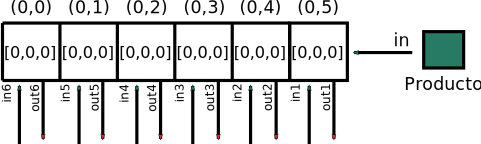
\includegraphics[width=0.8\textwidth]{CT-automata.pdf} 
  \caption{Autómata celular de la cinta transportadora.} 
  \label{fig:CT-automata} 
\end{figure}
\FloatBarrier


Los productos ingresan por la entrada \texttt{in} y se van desplazando hacia la izquierda a una velocidad representada por el tiempo entre ejecuciones de las reglas.

Para cada celda en este autómata celular importa solamente el valor de la celda anterior y el de la celda posterior. Por este motivo el vecindario está definido en la Figura~\ref{fig:CT-vecindario}.

\begin{figure}[h] 
  \centering 
  
\includegraphics[width=0.4\textwidth]{CT-vecindario.pdf} 
  \caption{Vecindario de la cinta transportadora.} 
  \label{fig:CT-vecindario} 
\end{figure}
\FloatBarrier

Cada elemento de la cinta transportadora está asociado a una columna en el inventario. A su vez, cada columna en el inventario tiene asignado un rango de fechas de vencimiento posibles, estando más hacia la izquierda las columnas asociadas a vencimientos más remotos.

Las consultas de lugar disponible en una columna del inventario se realizan enviando un valor de fecha de vencimiento imposible, en este caso igual a $-1$. El inventario debe responder con $0$ si no hay lugar en la columna por la que se consultó o un número no nulo en caso contrario. En caso que la respuesta del inventario sea que no hay lugar en la columna por la que se consultó entonces la cinta debe hacer avanzar al producto hacia la izquierda una posición más y volver a preguntar por la disponibilidad de espacio en el inventario.

Cada elemento en la cinta transportadora se representa con una tupla de tres elementos: \texttt{[ID columna, producto, indicador]}. El \texttt{ID columna} representa el rango de fechas de vencimiento asociados a la celda y a la columna respectiva del inventario. El elemento \texttt{producto} es el producto en sí y está representado por su fecha de vencimiento. Por último, el elemento \texttt{indicador} puede tener distintos significados dependiendo de su valor y los valores que puede tomar son: $0$, $1$ ó $2$. Si vale $1$ significa que el producto estaba listo para ser ubicado en la columna del inventario asociada a la celda actual de la cinta transportadora pero se recibió un mensaje indicando que no había lugar, si en cambio vale $2$ significa que ninguna de las columnas del inventario por las que se consultó tenía espacio y entonces ese producto permanecerá en la cinta transportadora.

Los elementos de las tuplas se acceden utilizando el signo de exclamación e indicando a continuación el elemento que se quiere acceder. Así por ejemplo el elemento $0$ o \texttt{ID columna} de la celda actual se accede mediante $(0,0)!0$.

Las reglas tienen la siguiente sintaxis: 
\begin{lstlisting}
rule : { resultado } { demora } { condicion }
\end{lstlisting}

Las reglas que representan a la descripción anterior y están asociadas a las células de este autómata celular se enumeran a continuación:

\begin{minipage}{1\textwidth}
	\centering
	\begin{lstlisting}
[cinta-reglas]
rule : { [(0,0)!0,(0,1)!1,0] } { 100 } { NOT isUndefined((0,1)!1) AND (0,1)!1 != 0 AND (0,1)!1 > (0,1)!0 + time/1000 }
rule : { [(0,0)!0,0,0] } { 100 } { NOT isUndefined((0,-1)!1) AND (0,0)!1 != 0 AND (0,0)!1 > (0,0)!0 + time/1000 AND (0,-1)!1 = 0 } 
rule : { [(0,0)!0,(0,1)!1,0] } { 100 } { (0,1)!2 = 1 }
rule : { [(0,0)!0,0,0] } { 100 } { (0,0)!2 = 1 AND NOT isUndefined((0,-1)!1) AND (0,-1)!1 = 0 }
rule : { [(0,0)!0,(0,0)!1,2] } { 100 } { (0,0)!2 = 1 AND (isUndefined((0,-1)!1) OR (0,-1)!1 != 0) }
rule : { [(0,0)!0,(0,0)!1+send(output,-1),0] } { 100 } { (0,0)!2 != 2 AND (0,0)!1 != 0 AND (0,0)!1 <= (0,0)!0 + time/1000 }
rule : { (0,0) } 0 { t }
	\end{lstlisting}
\end{minipage}

La primera regla pregunta si la celda que está a la derecha de la celda actual está definida: \texttt{NOT isUndefined((0,1)!1)}, tiene un producto: \texttt{(0,1)!1 != 0} y la fecha de vencimiento del producto es mayor que el \texttt{ID} de la columna \texttt{(0,1)!1 > (0,1)!0 + time/1000}. En caso que se cumpla se mueve el producto desde la celda de la derecha a la celda actual.

La segunda regla es el complemento de la primera, es decir, pregunta si la celda de la izquierda está definida: \texttt{NOT isUndefined((0,-1)!1)}, si está vacía: \texttt{(0,-1)!1 = 0}, si en la celda actual hay un producto y si su fecha de vencimiento es mayor que el \texttt{ID} de la columna: \texttt{(0,0)!1 > (0,0)!0 + time/1000}. Si se cumple, entonces se quita el producto de esta celda.

La tercera regla verifica si el elemento \texttt{indicador} de la tupla de la celda de la derecha es $1$. Si es así significa que la cinta consultó al inventario para mover ese producto y éste le respondió que no había lugar. Entonces lo que se hace es mover ese producto a la siguiente celda hacia la izquierda.

La cuarta regla es el complemento de la tercera regla, pregunta si el elemento \texttt{indicador} de la tupla de la celda actual es $1$ y si la celda de la izquierda está vacía. Si se cumple entonces quita al producto de esta celda.

La quinta regla se ejecuta cuando el producto no puede ser descargado en el inventario porque no hay lugar en las columnas que pregunta y alcanza el extremo izquierdo de la cinta transportadora. Esta condición se indica escribiendo un $2$ en el elemento \texttt{indicador} de la celda.

La sexta regla es la que permite hacer la consulta al inventario de si hay lugar en la columna correspondiente. Esta consulta se realiza enviando $-1$ por la salida asociada con la celda \texttt{outi} y la respuesta se espera por la entrada \texttt{ini}. Se puede ver que si el elemento \texttt{indicador} de la celda actual es $2$ entonces esta regla no se ejecuta, es decir, no se repite la consulta al inventario.

Finalmente, la séptima regla es la regla por omisión que es siempre verdadera pues debe existir siempre al menos una regla verdadera.

Asimismo, se definieron reglas que se ejecutan ante la aparición de las distintas entradas. Así, ante el arribo de un producto por la entrada \texttt{in} se ejecuta la siguiente regla:

\begin{minipage}{1\textwidth}
	\centering
	\begin{lstlisting}
[in-regla]
rule : { [(0,0)!0,portValue(thisPort),0] } { 1 } { t }
	\end{lstlisting}
\end{minipage}

Se observa que lo que se hace es copiar el producto que acaba de llegar en la celda conectada a la entrada \texttt{in}.

Finalmente, como se mencionó más arriba, cuando el producto llega a la celda que le corresponde en la cinta transportadora se genera una consulta al inventario para saber si existe lugar en la columna correspondiente. Las reglas que se evalúan cuando llega la respuesta son:

\begin{minipage}{1\textwidth}
	\centering
	\begin{lstlisting}
[inventario-regla]
rule : { [(0,0)!0,0+send(output,(0,0)!1),0] } { 1 } { portValue(thisPort)!=0 }
rule : { [(0,0)!0,(0,0)!1,1] } { 1 } { portValue(thisPort)=0 }
	\end{lstlisting}
\end{minipage}

Se puede ver que como se utiliza el comando \texttt{thisPort} esta regla es válida para todas las celdas de la cinta transportadora. Si la respuesta que recibe la celda de parte del inventario es no nula entonces se envía el producto por el mismo puerto por el que se realizó la consulta: \texttt{[(0,0)!0,0+send(output,(0,0)!1),0]} y se coloca un $0$ en su lugar. Si en cambio no hay lugar entonces se indica colocando un $1$ en el indicador de la tupla: \texttt{[(0,0)!0,(0,0)!1,1]}.

Este conjunto de reglas junto con la estructura graficada en la Figura~\ref{fig:CT-automata} definen el modelo de la cinta transportadora. Los links y la asignación de reglas se pueden ver en la siguiente definición dentro del archivo ".ma".

\begin{minipage}{1\textwidth}
	\centering
	\begin{lstlisting}
[cinta]
type : cell
dim : (1,6)
delay : transport
defaultDelayTime  : 0
border : nowrapped
neighbors : cinta(0,-1) cinta(0,0) cinta(0,1)
initialvalue : 0
initialCellsValue : cinta.val
in : in in1 in2 in3 in4 in5 in6
out : out1 out2 out3 out4 out5 out6
link : in in@cinta(0,5)
link : in1 in1@cinta(0,5)
link : in2 in2@cinta(0,4)
link : in3 in3@cinta(0,3)
link : in4 in4@cinta(0,2)
link : in5 in5@cinta(0,1)
link : in6 in6@cinta(0,0)
link : output@cinta(0,5) out1
link : output@cinta(0,4) out2
link : output@cinta(0,3) out3
link : output@cinta(0,2) out4
link : output@cinta(0,1) out5
link : output@cinta(0,0) out6
portintransition : in@cinta(0,5) in-regla
portintransition : in1@cinta(0,5) inventario-regla
portintransition : in2@cinta(0,4) inventario-regla
portintransition : in3@cinta(0,3) inventario-regla
portintransition : in4@cinta(0,2) inventario-regla
portintransition : in5@cinta(0,1) inventario-regla
portintransition : in6@cinta(0,0) inventario-regla
localtransition : cinta-reglas
	\end{lstlisting}
\end{minipage}

\subsection{Despacho de productos}\label{sec:DP}
Según lo descripto en la sección \ref{sec:AC} el despacho de productos es el encargado de extraer los productos del inventario propiamente dicho.
Su modelo estructural se muestra en la Figura~\ref{fig:DP-estructura}.

\begin{figure}[h] 
	\centering 
	\includegraphics[width=0.5\textwidth]{DP-estructura} 
	\caption{Modelo del despacho de productos.} 
	\label{fig:DP-estructura} 
\end{figure}

Conceptualmente se pueden dividir dos tipos de información que se propagarán por el modelo. Por un lado, el despachante que va buscando en qué columna tiene un producto para extraer (recordar que los productos se ordenan de forma que los más próximos a vencer se encuentran cerca de la salida) representado en la Figura~\ref{fig:DP-estructura} por un círculo de color rojo. Por otro, el producto en sí representado por un cuadrado de color verde. Ambos realizarán movimientos en direcciones opuestas, el despachante irá recorriendo el inventario hacia la izquierda buscando la primer columna con productos y, una vez que lo retira, el producto se moverá hacia la derecha en dirección a la salida.

Esta separación da origen a dos grupos (conceptuales) de reglas:
\begin{itemize}
	\item Reglas para movimiento de productos.
	\item Reglas para movimiento del despachante.
\end{itemize}

Ubicadas en ese orden estamos dando prioridad al movimiento de productos y por ende, si un pedido se realiza cuando el despachante no está en su puesto, es decir, cuando está buscando un producto, el pedido se pierde. El vecindario para el despacho de productos se corresponde con el utilizado para la cinta transportadora y se puede observar en la Figura~\ref{fig:CT-vecindario}. 

Las reglas se detallan a continuación:

\begin{minipage}{1\textwidth}
	\centering
	\begin{lstlisting}
[despacho-reglas]
% Con -1 pregunta al inventario si hay lugar

% Movimiento del producto sacado del inventario
% Las tres reglas sigueintes preguntan por >0 para no actuar con el pedido.
rule : { (0,-1) } 100 { not isUndefined((0,-1)!0) and (0,-1)!0>0 and (0,0)!0=0 }
rule : { [0,0] } 1 { not isUndefined((0,1)!0) and (0,1)!0>0 }
rule : { [0+send(output,(0,0)!0),0] } 1 { cellPos(1)=6 and (0,0)!0>0 }

% Movimiento del despachante buscando el producto
rule : {[-1+send(output,-1),0]} 100 { not isUndefined((0,1)!0) and (0,1)=[0,-1] and (0,0)!0=0 }
rule : {[0,0]} 1 { not isUndefined((0,-1)!0) and (0,-1)=[-1,0]}

% always true (condicion default)
rule : { (0,0) } 0 { t }
	\end{lstlisting}
\end{minipage}

Siendo respectivamente las primeras tres reglas responsables del movimiento del producto y con el siguiente significado:
\begin{enumerate}
	\item Copia el valor de la celda contigua a la izquierda si dicha celda existe y contiene un producto (i.e. su valor es $>0$), y si la celda en cuestión está vacía.
	\item Si el producto se movió a la derecha la celda se setea en 0
	\item Si llegó a la última celda de la derecha (oficina del despachante), la celda se pone en 0 y envía el producto por la salida de productos.
\end{enumerate}

Y las siguientes dos las responsables del movimiento del despachante, respectivamente:
\begin{enumerate}
	\item Se setea la celda en [-1,0] y envía la consulta de disponibilidad de productos en esa columna al inventario, si la celda próxima a la derecha está en estado de consulta fallida (ver a continuación), y si dicha celda existe.
	\item La celda se setea en 0 si el despachante se movió una posición hacia la izquierda (i.e. (0,-1)=[-1,0])
\end{enumerate}

Se utilizaron tuplas de dos posiciones para representar el estado de la celda. Esto permite marcar cuando un pedido fue realizado al inventario y éste último informa que en esa columna no hay disponibilidad, resultando en una consulta fallida, representada por el valor [0,-1] en la celda. Este es el caso donde el despachante deberá avanzar una columna más hacia la izquierda, según la primer regla de arriba, asociada al despachante.

Para terminar de definir el modelo, se deben especificar los comportamientos de los diferentes puertos, para ello se plantearon dos juegos de reglas. El primero para la entrada de pedidos, que simplemente copia el valor del pedido de productos (-1) en la celda correspondiente (oficina del despachante). El segundo para los valores que envía el inventario: por un lado  setea el estado de la celda en consulta fallida ([0,-1]) si el inventario devuelve 0, o por otro, copia el valor si el inventario devuelve un producto (valor $>0$). Dichas reglas se muestran a continuación:
Las velocidades del despachante y del producto se ajustaron seteando el tiempo de transición de una celda en otra en en 100 ms. Mientras que las salidas y entradas se setearon con una velocidad de 1 ms.

Para terminar de definir el modelo, se deben especificar los comportamientos de los diferentes puertos, para ello se plantearon dos juegos de reglas. El primero para la entrada de pedidos, que simplemente copia el valor del pedido de productos (-1) en la celda correspondiente (oficina del despachante). El segundo para los valores que envía el inventario: por un lado  setea el estado de la celda en consulta fallida ([0,-1]) si el inventario devuelve 0, o por otro, copia el valor si el inventario devuelve un producto (valor >0). Dichas reglas se muestran a continuación:

\begin{minipage}{1\textwidth}
	\centering
	\begin{lstlisting}
[pedidosIn-regla]
rule : { [0,portValue(thisPort)] } 1 { portValue(thisPort)=-1 }

[ins-regla]
rule : { [0,-1] } 1 { portValue(thisPort)=0 }
rule : { [portValue(thisPort),0] } 1 { portValue(thisPort)>0 }
	\end{lstlisting}
\end{minipage}

Este conjunto de reglas con la estructura graficada en la Figura~\ref{fig:DP-estructura} definen el modelo del despacho de productos. Los links y la asignación de reglas se pueden ver en la siguiente definición dentro del archivo ".ma"

\begin{minipage}{1\textwidth}
	\centering
	\begin{lstlisting}
[despacho]
type : cell
dim : (1,7)
delay : transport
defaultDelayTime  : 0
border : nowrapped
neighbors : despacho(0,-1) despacho(0,0) despacho(0,1)
initialvalue : 0
initialCellsValue : despacho.val
in : pedidosIn in1 in2 in3 in4 in5 in6
out : pedidosOut out1 out2 out3 out4 out5 out6
link : pedidosIn in@despacho(0,6)
link : in6 in@despacho(0,5)
link : in5 in@despacho(0,4)
link : in4 in@despacho(0,3)
link : in3 in@despacho(0,2)
link : in2 in@despacho(0,1)
link : in1 in@despacho(0,0)
link : output@despacho(0,6) pedidosOut
link : output@despacho(0,5) out6
link : output@despacho(0,4) out5
link : output@despacho(0,3) out4
link : output@despacho(0,2) out3
link : output@despacho(0,1) out2
link : output@despacho(0,0) out1
portintransition : in@despacho(0,6) pedidosIn-regla
portintransition : in@despacho(0,5) ins-regla
portintransition : in@despacho(0,4) ins-regla
portintransition : in@despacho(0,3) ins-regla
portintransition : in@despacho(0,2) ins-regla
portintransition : in@despacho(0,1) ins-regla
portintransition : in@despacho(0,0) ins-regla
localtransition : despacho-reglas
\end{lstlisting}
\end{minipage}


\section{Modelado y Simulación}
\subsection{Pruebas parciales}
\subsubsection{Cinta Transportadora}

Para este ejemplo se utilizó una cinta transportadora de $6$ celdas. El tiempo entre ejecuciones de las reglas en las transiciones locales se configuró en $100~\textrm{ms}$, mientras que el tiempo en las reglas de las transiciones en los puertos de entrada se configuró en $1~\textrm{ms}$. Con el primer tiempo se modeliza la velocidad de avance de la cinta transportadora.

Los valores iniciales de las celdas se configuraron mediante el archivo \texttt{cinta.val} cuyo contenido se muestra a continuación:

\begin{minipage}{1\textwidth}
	\centering
	\begin{lstlisting}
(0,0) = [0.6,0  ,0]
(0,1) = [0.5,0  ,0]
(0,2) = [0.4,0  ,0]
(0,3) = [0.3,0  ,0]
(0,4) = [0.2,0  ,0]
(0,5) = [0.1,0.3,0]
	\end{lstlisting}
\end{minipage}

Se observa que cada celda tiene asociada una tupla de tres elementos. El primer elemento de estas tuplas identifica a la fecha de vencimiento de la celda. Esta fecha de vencimiento se mantiene fija a lo largo de la simulación aunque al momento de comparar la fecha de vencimiento de un producto con el de la celda a esta última se le suma el tiempo actual \texttt{time/1000}.

Los eventos de entrada: a) arribo de productos a la cinta y b) respuestas del inventario se manejan mediante el archivo \texttt{cinta.ev} cuyo contenido se meustra a continuación:

\begin{minipage}{1\textwidth}
	\centering
	\begin{lstlisting}
00:00:00:111 in2 0
00:00:00:221 in3 1
00:05:00:000 in  300.4
00:06:00:000 in3 1
00:10:00:000 in  600.2
00:11:00:000 in2 1
00:15:00:000 in  900.5
00:16:00:000 in3 0
00:17:00:000 in4 0
00:18:00:000 in5 0
00:19:00:000 in6 0
	\end{lstlisting}	
\end{minipage}

Para analizar el comportamiento del autómata celular que utiliza las reglas antes mencionadas y la secuencia de eventos de entrada del archivo \texttt{cinta.ev} se ejecutó el simulador con el parámetro \texttt{-v} de modo de tener una salida \textit{verbosa}. El primer producto que ingresa en la cinta lo hace mediante el archivo \texttt{cinta.val}. La salida de la prueba es la siguiente:

\begin{minipage}{1\textwidth}
	\centering
	\begin{lstlisting}
0 / L / Y / 00:00:00:100:0 / out2 /  -1.0 /
0 / L / X / 00:00:00:111:0 /  in2 /   0.0 /
0 / L / Y / 00:00:00:212:0 / out3 /  -1.0 /
0 / L / X / 00:00:00:221:0 /  in3 /   1.0 /
0 / L / Y / 00:00:00:221:0 / out3 /   0.3 /
0 / L / X / 00:05:00:000:0 /   in / 300.4 /
0 / L / Y / 00:05:00:201:0 / out3 /  -1.0 /
0 / L / X / 00:06:00:000:0 /  in3 /   1.0 /
0 / L / Y / 00:06:00:000:0 / out3 / 300.4 /
0 / L / X / 00:10:00:000:0 /   in / 600.2 /
0 / L / Y / 00:10:00:101:0 / out2 /  -1.0 /
0 / L / X / 00:11:00:000:0 /  in2 /   1.0 /
0 / L / Y / 00:11:00:000:0 / out2 / 600.2 /
0 / L / X / 00:15:00:000:0 /   in / 900.5 /
0 / L / Y / 00:15:00:201:0 / out3 /  -1.0 /
0 / L / X / 00:16:00:000:0 /  in3 /   0.0 /
0 / L / Y / 00:16:00:101:0 / out4 /  -1.0 /
0 / L / X / 00:17:00:000:0 /  in4 /   0.0 /
0 / L / Y / 00:17:00:101:0 / out5 /  -1.0 /
0 / L / X / 00:18:00:000:0 /  in5 /   0.0 /
0 / L / Y / 00:18:00:101:0 / out6 /  -1.0 /
0 / L / X / 00:19:00:000:0 /  in6 /   0.0 /
	\end{lstlisting}	
\end{minipage}

Esta salida se obtuvo del archivo \texttt{log} del modelo \textit{top} reteniendo solamente los eventos de entrada (X) y salida (Y). El primer producto ingresa a la cinta durante la inicialización y por ese motivo no aparece aquí. Ese primer producto tiene una fecha de vencimiento de $0.3$. En el tiempo $0$ se evalúan todas las celdas y el producto avanza una celda hacia la izquierda alcanzando la celda $(0,4)$ de la Figura~\ref{fig:CT-automata}. La siguiente ejecución de las reglas se produce a los $100~\textrm{ms}$ y sólo se evalúan las celdas en el vecindario inverso de las celdas que sufrieron modificaciones en el paso anterior. En este paso el producto no avanza un casillero más hacia la izquierda pues en la comparación de \texttt{(0,0)!1} con \texttt{(0,0)!0 + time/1000} de las primera y segunda regla el producto se queda en la celda $(0,4)$ cuyo campo \texttt{ID} es $0.2$. Entonces en este paso se consulta al inventario si hay lugar disponible en la columna conectada a la salida \texttt{out2} enviando un $-1$ por el puerto de salida. Un tiempo después llega la respuesta del inventario indicando con un $0$ que no hay lugar, entonces el producto avanzará una posición en la celda. Se repite la consulta al inventario pero esta vez desde la salida \texttt{out3}. Al tiempo llega la respuesta del inventario indicando que hay lugar e instantáneamente la cinta descarga el producto por la salida. Luego de un tiempo arriba un producto de valor de fecha de vencimiento $300.4~\textrm{ms}$. Este producto avanza en la cinta hasta la posición $(0,3)$, consulta si hay lugar en el inventario y se descarga allí. De igual manera se procede con el producto que ingresa a la cinta a continuación de valor de fecha de vencimiento $600.2~\textrm{ms}$. Finalmente, el último producto de valor $900.5~\textrm{ms}$ que avanza hasta la celda $(0,3)$ y consulta al inventario, ante la respuesta de éste el producto avanza una posición más en la cinta transportadora y vuelve a consultar. Esta operación se repite y el producto alcanza el final de la cinta transportadora y ante la falta de lugar en el inventario entonces el producto permanece en la cinta transportadora.

Para tener mayor detalle de la ejecución de las reglas se puede observar la salida del simulador en modo \textit{verboso}. Allí se puede observar que cada vez que se evalúa una regla en una celda se determina su vecindario inverso y de éste se determinan las celdas que podrían verse afectadas por un cambio en el valor de dicha celda. De esta manera no están ejecutándose siempre todas las reglas para todas las celdas. Esto se puede observar en el siguiente extracto de la salida (donde para faciliar la legibilidad se quitaron algunas líneas):

\begin{minipage}{1\textwidth}
	\centering
	\begin{lstlisting}
+-----------------------------------------------------+
New Eval: in-regla - 00:05:00:000:0 - cinta(0,5)
Eval: PortIn Reference(in) = 300.4
Eval: SendToNCPort Reference(out, [0.1, 300.4, 0]) at time 00:05:00:000:0
+-----------------------------------------------------+
New Eval: cinta-reglas - 00:05:00:001:0 - cinta(0,4)
Eval: SendToNCPort Reference(out, [0.2, 300.4, 0]) at time 00:05:00:001:0
+-----------------------------------------------------+
New Eval: cinta-reglas - 00:05:00:001:0 - cinta(0,5)
Eval: SendToNCPort Reference(out, [0.1, 0, 0]) at time 00:05:00:001:0
+-----------------------------------------------------+
New Eval: cinta-reglas - 00:05:00:101:0 - cinta(0,3)
Eval: SendToNCPort Reference(out, [0.3, 300.4, 0]) at time 00:05:00:101:0
+-----------------------------------------------------+
New Eval: cinta-reglas - 00:05:00:101:0 - cinta(0,4)
Eval: SendToNCPort Reference(out, [0.2, 0, 0]) at time 00:05:00:101:0
+-----------------------------------------------------+
New Eval: cinta-reglas - 00:05:00:101:0 - cinta(0,5)
Eval: SendToNCPort Reference(out, [0.1, 0, 0]) at time 00:05:00:101:0
+-----------------------------------------------------+
New Eval: cinta-reglas - 00:05:00:201:0 - cinta(0,2)
Eval: SendToNCPort Reference(out, [0.4, 0, 0]) at time 00:05:00:201:0
+-----------------------------------------------------+
New Eval: cinta-reglas - 00:05:00:201:0 - cinta(0,3)
Eval: SendToPort Reference(output, -1) at time 00:05:00:201:0
Eval: SendToNCPort Reference(out, [0.3, 300.4, 0]) at time 00:05:00:201:0
+-----------------------------------------------------+
New Eval: cinta-reglas - 00:05:00:201:0 - cinta(0,4)
Eval: SendToNCPort Reference(out, [0.2, 0, 0]) at time 00:05:00:201:0
+-----------------------------------------------------+
New Eval: cinta-reglas - 00:05:00:201:0 - cinta(0,5)
Eval: SendToNCPort Reference(out, [0.1, 0, 0]) at time 00:05:00:201:0
+-----------------------------------------------------+
New Eval: inventario-regla - 00:06:00:000:0 - cinta(0,3)
Eval: PortIn Reference(in3) = 1
Eval: SendToPort Reference(output, 300.4) at time 00:06:00:000:0
Eval: SendToNCPort Reference(out, [0.3, 0, 0]) at time 00:06:00:000:0
	\end{lstlisting}	
\end{minipage}

En esta prueba se observa que se produce un evento de entrada en $00:05:00:000$ que modifica el estado de la celda (0,5). Este evento es el ingreso de un producto de fecha de vencimiento $300.4$. La demora de las reglas asociadas con entradas es de $1~\textrm{ms}$. En $00:05:00:001$ se determina el vecindario inverso de la celda $(0,5)$, que consiste en las celdas $(0,4)$ y $(0,5)$, y se evalúa cómo repercuten los cambios en la celda $(0,5)$. Para las celdas en este vecindario se ejecutan la primera y segunda regla y el producto avanza a la celda $(0,4)$ y se quita de la $(0,5)$. Las reglas locales se ejecutan cada $100~\textrm{ms}$, por lo tanto en el tiempo $00:05:00:101$ se evalúa el vecindario inverso de las celdas que sufrieron cambios en al paso anterior. Este vecindario inverso está compuesto por las celdas $(0,3)$, $(0,4)$ y $(0,5)$. En este paso el producto avanza una celda más hacia la izquierda pasando a la celda $(0,3)$. Nuevamente se esperan $100~\textrm{ms}$ para volver a evauar las reglas y en este caso se determina que la celda $(0,3)$ es la que le corresponde al producto y entonces se consulta inventario por la disponibilidad de lugar. Se puede observar que como el valor de las celdas evaluadas en $00:05:00:201$ no cambió entonces no se vuelven a evaluar las reglas locales. La respuesta del inventario llega a la celda $(0,3)$ en el tiempo $00:06:00:000$.

\subsubsection{Inventario}
Las pruebas de este módulo por

\subsubsection{Despacho de Productos}
Para la prueba de este módulo también se procedió a excitarlo con un archivo de eventos ".ev", conteniendo los pedidos de productos y las respuestas del inventario. Se tuvo especial cuidado en generar las respuestas del inventario en los momentos adecuados a la salida de consultas a las columnas. Considerando que la asignación de los valores de las reglas tiene un retraso de 1 (velocidad del despachante).

\begin{minipage}{1\textwidth}
	\centering
	\begin{lstlisting}
00:01:00:000 pedidosIn -1
00:01:00:103 in6 0
00:01:00:206 in5 0
00:01:00:309 in4 0
00:01:00:412 in3 300.4
00:01:01:000 pedidosIn -1
00:01:01:103 in6 0
00:01:01:206 in5 0
00:01:01:309 in4 0
00:01:01:412 in3 0
00:01:01:515 in2 0
00:01:01:618 in1 600.2
00:02:00:000 pedidosIn -1
00:02:00:103 in6 900.5
	\end{lstlisting}	
\end{minipage}

Ante este estímulo, el comportamiento que se espera es el siguiente:
\begin{enumerate}
	\item En el tiempo 00:01:00:000 se recibe un evento de pedido de producto.
	\item Luego de 1 ms el pedido se registra en la oficina del despachante (celda (0,5)).
	\item Luego de 100 ms, el despachante camina hasta la primera columna del inventario (celda (0,5)) y hace el pedido al inventario.
	\item En el tiempo 00:01:00:103 el inventario responde que no hay productos en esa columna.
	\item Luego de 1 ms más el despachante camina una columna más y repite el pedido.
	\item Se repite el proceso con sus respectivos tiempos hasta que el despachante llega a la columna 3 (celda (0,2)) donde el inventario en tiempo 00:01:00:412 responde con un producto con fecha de caducidad 600.2 (recordar que el control de calidad se realiza por un modelo atómico mostrado en el TP1).
	\item El producto se debe desplazar hacia la derecha a 100 ms por celda hasta salir por el puerto de salida de pedidos.
	\item El proceso se repite ante una llegada de un pedido en el tiempo 00:01:01:000. Pero el despachante debe llegar hasta la primer columna para encontrar un producto.
	\item Finalmente el proceso se repite en el tiempo 00:02:00:000 pero el inventario dispone de producto en la columna más cercana al despachante (celda (0,5)). Por lo que el recorrido del despachante es solamente de una posición.
\end{enumerate}

Para verificar el comportamiento esperado anterior, se procedió a analizar los archivos logs generados. Filtrando con el comando \textit{grep}, y conociendo la nomenclatura de los mensajes se puede analizar el comportamiento.
Para la salida del top-model podemos observar:

\begin{minipage}{1\textwidth}
	\centering
	\begin{lstlisting}
0 / L / Y / 00:01:00:001:0 / despacho(01) / out6 /     -1.00000 / top(09)
0 / L / Y / 00:01:00:104:0 / despacho(01) / out5 /     -1.00000 / top(09)
0 / L / Y / 00:01:00:207:0 / despacho(01) / out4 /     -1.00000 / top(09)
0 / L / Y / 00:01:00:310:0 / despacho(01) / out3 /     -1.00000 / top(09)
0 / L / Y / 00:01:00:813:0 / despacho(01) / pedidosout /    300.40000 / top(09)
0 / L / Y / 00:01:01:001:0 / despacho(01) / out6 /     -1.00000 / top(09)
0 / L / Y / 00:01:01:104:0 / despacho(01) / out5 /     -1.00000 / top(09)
0 / L / Y / 00:01:01:207:0 / despacho(01) / out4 /     -1.00000 / top(09)
0 / L / Y / 00:01:01:310:0 / despacho(01) / out3 /     -1.00000 / top(09)
0 / L / Y / 00:01:01:413:0 / despacho(01) / out2 /     -1.00000 / top(09)
0 / L / Y / 00:01:01:516:0 / despacho(01) / out1 /     -1.00000 / top(09)
0 / L / Y / 00:01:02:219:0 / despacho(01) / pedidosout /    600.20000 / top(09)
0 / L / Y / 00:02:00:001:0 / despacho(01) / out6 /     -1.00000 / top(09)
0 / L / Y / 00:02:00:204:0 / despacho(01) / pedidosout /    900.50000 / top(09)

	\end{lstlisting}	
\end{minipage}

Donde se observa que 100 ms después de cada respuesta del inventario se cursa un pedido a la columna siguiente. Por otro lado se observa que el producto sale correctamente por la salida \textit{pedidosOut} 503 ms después de haber entrado en el despacho, tal como fue previsto. Se observa coherencia también en los casos siguientes, con un tiempo de demora en la salida proporcional a la distancia recorrida por el despachante para encontrar un producto en el inventario.

\section{Conclusiones}

A lo largo del desarrollo del trabajo práctico con la herramienta CD++ en su versión \textit{standalone} se encontraron algunos inconvenientes: a) cuando se incluye un bloque generador se genera un error que indica que el bloque no está registrado, b) cuando se ejecuta el simulador avanzado con el parámetro \texttt{-r} se produce una excepción y se aborta la ejecución, c) no existe un visualizador para el simulador avanzado ya que los que hay (\textit{drawlog} y \textit{webviewer}) no permiten representar tuplas y d) el archivo de salida generado por el simulador con la opción \texttt{-o} genera un archivo vacío. Esto último dificulta el ensayo de los autómatas celulares. En lugar de utilizar tres autómatas celulares este trabajo podría haberse resuelto utilizando tan solo uno y definiendo tres zonas cada una con sus reglas. Sin embargo, en la versión avanzada del simulador nos recomendaron no utilizar zonas ya que no están aún debidamente probadas. No obstante los comentarios anteriores, la versión avanzada del simulador presenta como ventaja la incorporación de tuplas que simplifica los vecindarios a utilizar y da mayor flexibilidad.

\appendix
\section{Código Implementado}

\url{https://github.com/TwinT/DEVS-Inventario}

% Please don't exchange the bibliographystyle style
\bibliographystyle{IEEEtran.bst}
% AUTHOR: Include your bib file here
\bibliography{IEEEexample}

\end{document}

